\section{How it's different from Word}
    \subsection{WYSIWYG - What You See Is What You Get}
        You may be familiar with the challenge that is using Word to write equations even as simple as those in Figure \ref{fig:word}.

        \begin{figure}[h]
            \centering
            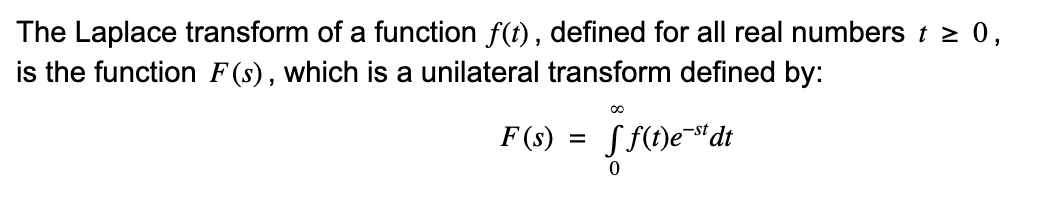
\includegraphics[scale=0.8]{figures/word.png}
            \caption{Word, an example of What You See Is What You Get}
            \label{fig:word}
        \end{figure}

        You may have tried to copy similar text and ended up with broken formatting --- mistached fonts, bad math formulas, etc.
        That's because this is \emph{rich} text, meaning the text you see contains all the information we have, like font, size, and so on.
        Popular word processing software, like Word, Pages, and so on, take this one step further to include a document's structure, leading to what is often called ``What You See Is What You Get'', or WYSIWYG for short.

        While there is a place for WYSIWYG editors, think of them as focused on producing text, and everything else is secondary.
        Good typesetting, well drawn diagrams, etc are absolutely essential for academic papers, so we use more specialised software that handles it more precisely.

    \subsection{Typesetting}
        \LaTeX, pronounced either \emph{lah-tec} or \emph{lay-tec}, is a collection of separate programmes which takes \emph{plain} text and instructions, then compiles them into a beautifully typeset document.
        The most important of these programmes is \TeX{}, which is responsible for the typesetting.

        The basic premise is that we focus on creating plain text content with the use of \LaTeX, which behind-the-scenes uses \TeX{} to handle the document's structure, fonts, drawings and so on.
        With structure and content being completely separate, it is easy to, for example, take several articles and create a uniform layout/look to them for a journal.
        But possibly the main reason why \TeX{} and \LaTeX{} became the standard in academia is the simplicity to write mathematical expressions.

        In summary, the main motivators for using \LaTeX{} are:
        \begin{enumerate}
            \item Beautifully written documents. While you can control fonts, margins, spacing, etc., they can be left to the specialists behind \TeX.  
            \item Easy bibliography management, citations and cross-references.
            \item Easily typed equations and graphs. Even complicated maths can be easily organised and written.
        \end{enumerate}

        Let's go back to our example, and see how it would be created with \LaTeX:
        \lstinputlisting[language=TeX, label=ls:Laplace, caption=Example document written with \LaTeX]{files/introduction/example1.tex}
        Which gets compiled into:\\
        The Laplace transform of a function $f(t)$, defined for all real numbers $t \geq 0$ is the function $F(s)$, which is a unilateral transform defined by:
        \begin{equation*}
            F(s) = \int_0^\infty f(t)e^{-st} dt
        \end{equation*}

        ---
        
        If you are familiar with programming, this may remind you of a \emph{markup} language, and that's exactly what it is!
        In short, we have a plain text file saved in \texttt{.tex} that contains 1) Information on what is needed for compilation into a \texttt{.pdf}, and 2) The document's contents.

        Another example is how to include figures into a document.
        If you are used to a graphical interface, you usually click a few buttons, then tinker with positioning and how text wraps around the figure.
        In contrast, with \LaTeX{} we simply issue a command and give it some options, like so:
        \begin{lstlisting}
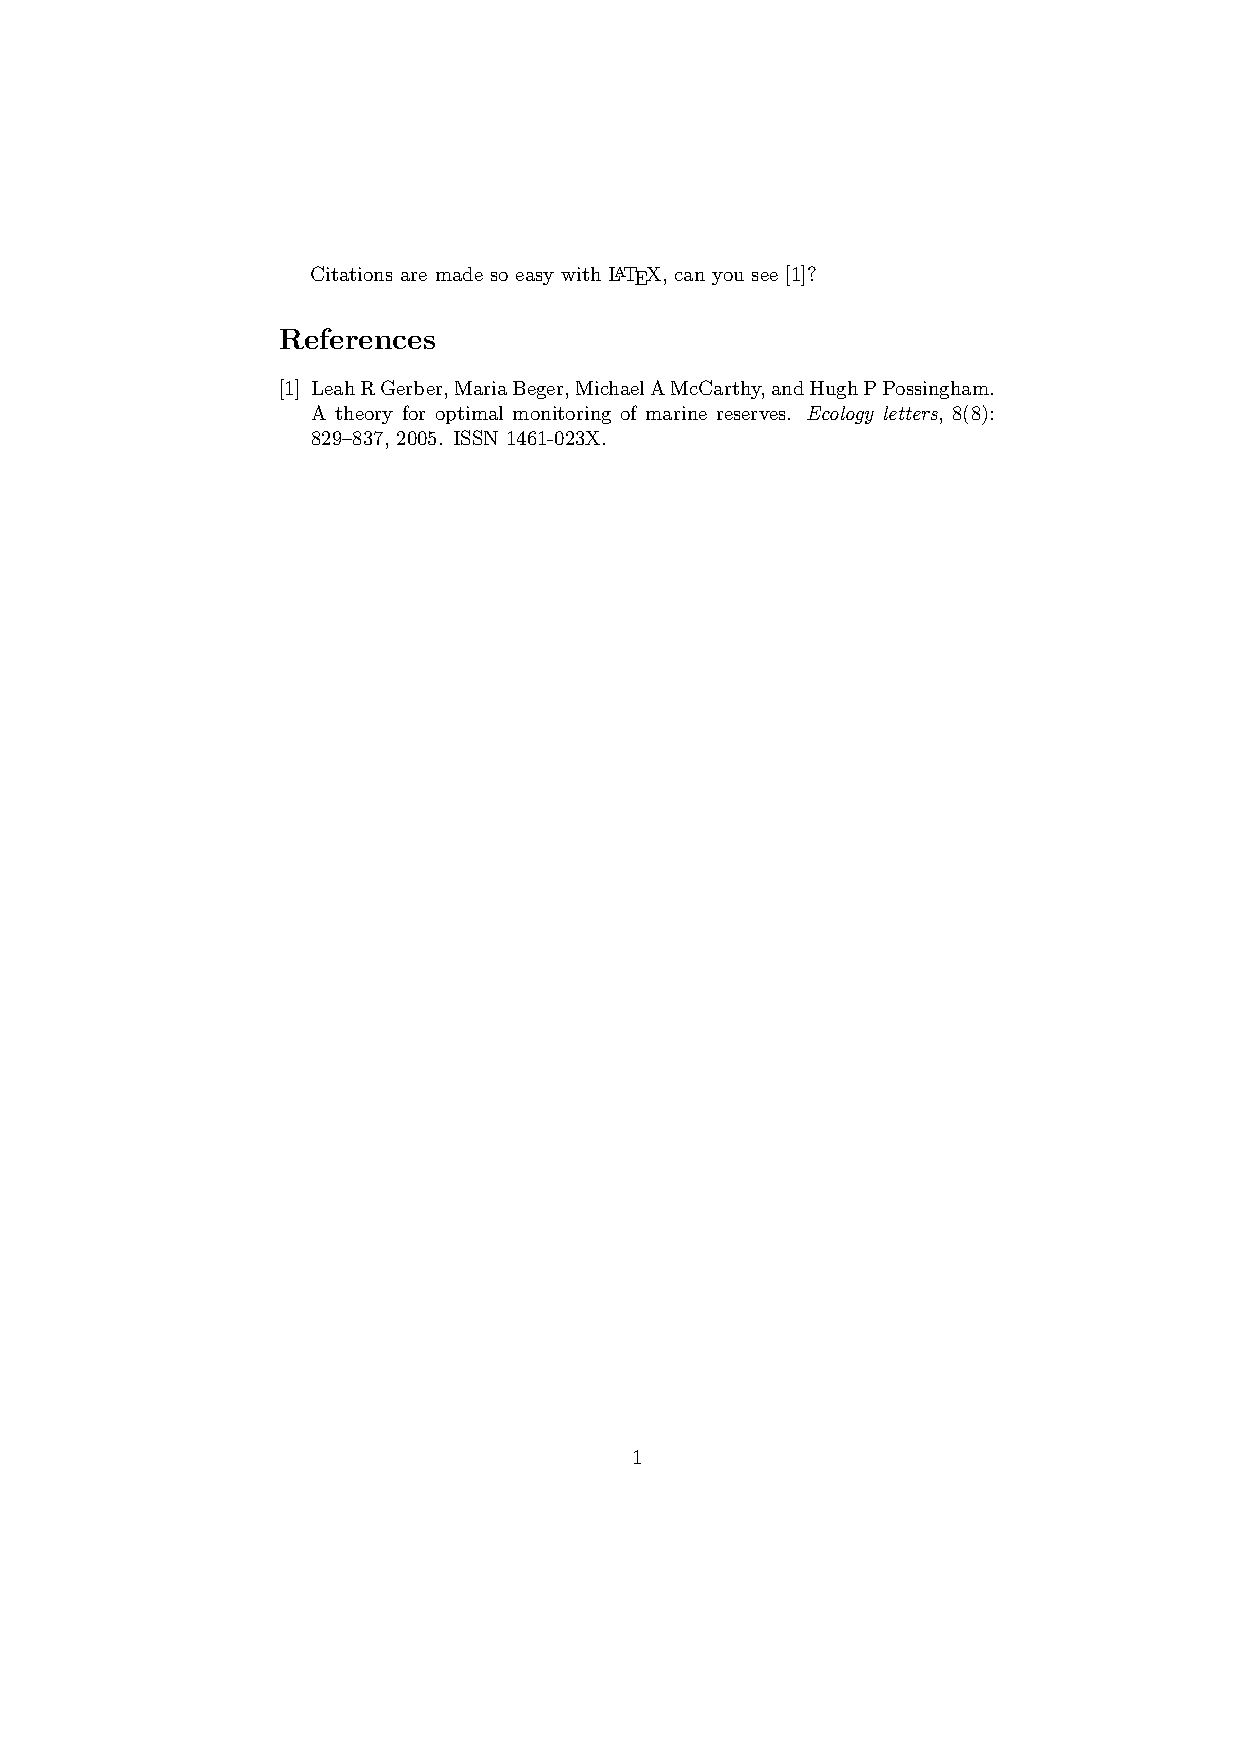
\includegraphics[width=0.5\textwidth]{figures/example.png}
        \end{lstlisting}
        This may seem verbose, but bear in mind that typing a line of code with auto-complete, suggestions, etc is often much quicker than interacting with a graphical interface.

        Let's briefly explore some key \LaTeX{} concepts.
\section{Markup language}
    Sentences are written in plain text, but most of LaTeX's power comes from the use of its \emph{markups}.
    A backslash, \verb|\|, followed by a word indicates a markup; like \verb|\alpha| producing \( \alpha \) or \verb|\pagebreak| creating a page break.
    
    Curly brackets, \verb|{}|, indicate an \emph{argument}, and square brackets \verb|[]| (optionally) provide options.
    So \verb|\section{Introduction}| would create an Introduction header at a \texttt{section} level, similar to a H1 header in Word.
    \verb|\includegraphics{}|, as we saw earlier, includes the graphic given as an argument.

    Generally, markups are used to either create \emph{environments}, give instructions/commands, or utilise variables \footnotemark.
    \footnotetext{This division is completely arbitrary, as you may notice from the syntax, but you may find it helpful to think of it this way.}

    \paragraph{Environments:}
    introduce some kind of formatting, such as where the document begins, lists, math mode or more complicated things.
    With very few exceptions, environments have the following format:
        
    \begin{lstlisting}
\begin{environment-name}[options]
    ...
\end{environment-name}
    \end{lstlisting}
        
    In our example, we created both the required \texttt{document} environment, and the math display \texttt{equation*}.
        
    \paragraph{Instructions/commands:}
    define some feature of the document. This ranges from breaking a page, to creating double-spacing, defining the document's class, and much more. In our example you can see:

    \verb|\documentclass[...]{article}|
        
    \paragraph{Variables:}
    range from greek letters to the integral sign to a whole expression.
    Some examples seen are \verb|\geq| (\textbf{g}reater or \textbf{eq}ual, \( \geq \)) and \verb|\int| ($\int$).
    Intuitively, \verb|\alpha| results in $\alpha$, and you can even create your own variables!
        
    \paragraph{Note:}
    Like other programming languages, there are certain reserved characters with predefined meaning, such as \verb|\|, \verb|{|, \verb|}|, \verb|&| and a few others.
    To use the literal curly brackets, ampersand, etc we would need to \emph{escape} them.
    Conveniently, this is done with a backslash (\verb|\|), so feel free to think of them as variables: \verb|\{|, \verb|\}| and \verb|\&|.

\section{Packages}
    You may have noticed that \verb|\usepackage{amsmath}| was not mentioned as an instruction the previous section. That's because packages are worth mentioning on their own.

    Packages add features to our document, similar to \emph{import} in most programming languages.
    \verb|amsmath| gives us a wide array of maths tools, but there are packages for drawing, graphing, colouring, better management of bibliography, easier organisation of your files, and so on.
    
\section{Compilation}
    As mentioned previously, \LaTeX\ documents are written in plain text with a set of instructions.
    This means that our \texttt{.tex} files can be written in any text editing software \verb|.tex|, and to produce the output \verb|.pdf|, it needs to be \emph{compiled}.

    You may spend a lot of time scratching your head, wondering what is wrong with your code and why it's not compiling.
    We very specifically will avoid most of the programming side of \TeX, which is a kind of macro expansion language.
    You will still run into some challenges, but they tend to be about forgetting brackets, rather than bugs causing unexpected behaviour.

    We are not going to focus on the various compilers, and just use \texttt{latexmk}, or whichever is default in your \LaTeX{} distribution.
    The good news is that the recommended IDEs (\textbf{I}ntegrated \textbf{D}evelopment \textbf{E}nvironments) handle the compilation for us and have features to help spot mistakes.